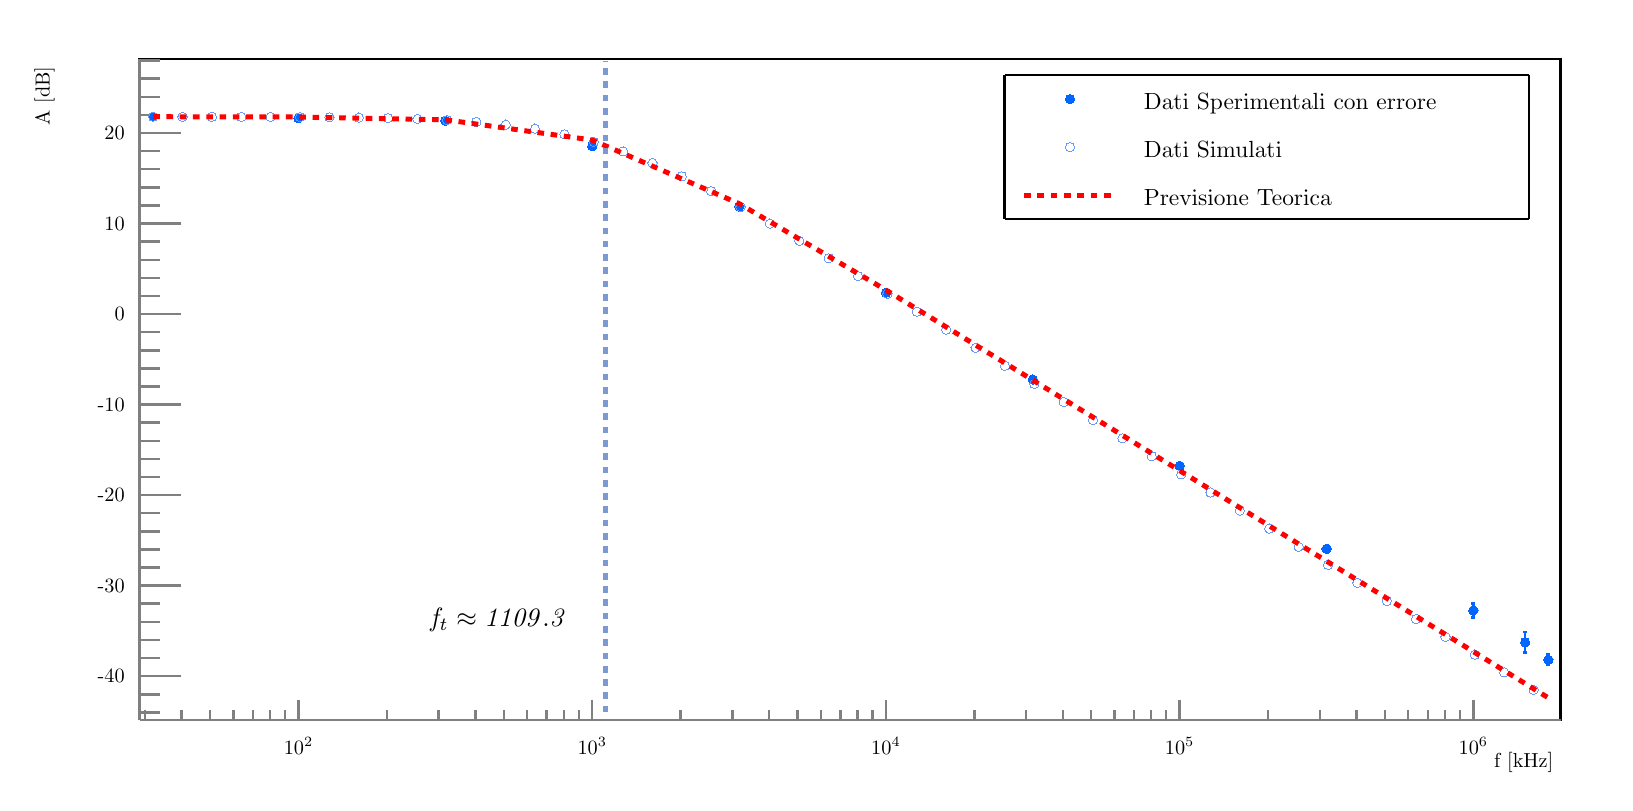
\begin{tikzpicture}
\pgfdeclareplotmark{cross} {
\pgfpathmoveto{\pgfpoint{-0.3\pgfplotmarksize}{\pgfplotmarksize}}
\pgfpathlineto{\pgfpoint{+0.3\pgfplotmarksize}{\pgfplotmarksize}}
\pgfpathlineto{\pgfpoint{+0.3\pgfplotmarksize}{0.3\pgfplotmarksize}}
\pgfpathlineto{\pgfpoint{+1\pgfplotmarksize}{0.3\pgfplotmarksize}}
\pgfpathlineto{\pgfpoint{+1\pgfplotmarksize}{-0.3\pgfplotmarksize}}
\pgfpathlineto{\pgfpoint{+0.3\pgfplotmarksize}{-0.3\pgfplotmarksize}}
\pgfpathlineto{\pgfpoint{+0.3\pgfplotmarksize}{-1.\pgfplotmarksize}}
\pgfpathlineto{\pgfpoint{-0.3\pgfplotmarksize}{-1.\pgfplotmarksize}}
\pgfpathlineto{\pgfpoint{-0.3\pgfplotmarksize}{-0.3\pgfplotmarksize}}
\pgfpathlineto{\pgfpoint{-1.\pgfplotmarksize}{-0.3\pgfplotmarksize}}
\pgfpathlineto{\pgfpoint{-1.\pgfplotmarksize}{0.3\pgfplotmarksize}}
\pgfpathlineto{\pgfpoint{-0.3\pgfplotmarksize}{0.3\pgfplotmarksize}}
\pgfpathclose
\pgfusepathqstroke
}
\pgfdeclareplotmark{cross*} {
\pgfpathmoveto{\pgfpoint{-0.3\pgfplotmarksize}{\pgfplotmarksize}}
\pgfpathlineto{\pgfpoint{+0.3\pgfplotmarksize}{\pgfplotmarksize}}
\pgfpathlineto{\pgfpoint{+0.3\pgfplotmarksize}{0.3\pgfplotmarksize}}
\pgfpathlineto{\pgfpoint{+1\pgfplotmarksize}{0.3\pgfplotmarksize}}
\pgfpathlineto{\pgfpoint{+1\pgfplotmarksize}{-0.3\pgfplotmarksize}}
\pgfpathlineto{\pgfpoint{+0.3\pgfplotmarksize}{-0.3\pgfplotmarksize}}
\pgfpathlineto{\pgfpoint{+0.3\pgfplotmarksize}{-1.\pgfplotmarksize}}
\pgfpathlineto{\pgfpoint{-0.3\pgfplotmarksize}{-1.\pgfplotmarksize}}
\pgfpathlineto{\pgfpoint{-0.3\pgfplotmarksize}{-0.3\pgfplotmarksize}}
\pgfpathlineto{\pgfpoint{-1.\pgfplotmarksize}{-0.3\pgfplotmarksize}}
\pgfpathlineto{\pgfpoint{-1.\pgfplotmarksize}{0.3\pgfplotmarksize}}
\pgfpathlineto{\pgfpoint{-0.3\pgfplotmarksize}{0.3\pgfplotmarksize}}
\pgfpathclose
\pgfusepathqfillstroke
}
\pgfdeclareplotmark{newstar} {
\pgfpathmoveto{\pgfqpoint{0pt}{\pgfplotmarksize}}
\pgfpathlineto{\pgfqpointpolar{44}{0.5\pgfplotmarksize}}
\pgfpathlineto{\pgfqpointpolar{18}{\pgfplotmarksize}}
\pgfpathlineto{\pgfqpointpolar{-20}{0.5\pgfplotmarksize}}
\pgfpathlineto{\pgfqpointpolar{-54}{\pgfplotmarksize}}
\pgfpathlineto{\pgfqpointpolar{-90}{0.5\pgfplotmarksize}}
\pgfpathlineto{\pgfqpointpolar{234}{\pgfplotmarksize}}
\pgfpathlineto{\pgfqpointpolar{198}{0.5\pgfplotmarksize}}
\pgfpathlineto{\pgfqpointpolar{162}{\pgfplotmarksize}}
\pgfpathlineto{\pgfqpointpolar{134}{0.5\pgfplotmarksize}}
\pgfpathclose
\pgfusepathqstroke
}
\pgfdeclareplotmark{newstar*} {
\pgfpathmoveto{\pgfqpoint{0pt}{\pgfplotmarksize}}
\pgfpathlineto{\pgfqpointpolar{44}{0.5\pgfplotmarksize}}
\pgfpathlineto{\pgfqpointpolar{18}{\pgfplotmarksize}}
\pgfpathlineto{\pgfqpointpolar{-20}{0.5\pgfplotmarksize}}
\pgfpathlineto{\pgfqpointpolar{-54}{\pgfplotmarksize}}
\pgfpathlineto{\pgfqpointpolar{-90}{0.5\pgfplotmarksize}}
\pgfpathlineto{\pgfqpointpolar{234}{\pgfplotmarksize}}
\pgfpathlineto{\pgfqpointpolar{198}{0.5\pgfplotmarksize}}
\pgfpathlineto{\pgfqpointpolar{162}{\pgfplotmarksize}}
\pgfpathlineto{\pgfqpointpolar{134}{0.5\pgfplotmarksize}}
\pgfpathclose
\pgfusepathqfillstroke
}
\definecolor{c}{rgb}{1,1,1};
\draw [color=c, fill=c] (0,0) rectangle (20,9.5746);
\draw [color=c, fill=c] (1.39683,0.787302) rectangle (19.4413,9.18095);
\definecolor{c}{rgb}{0,0,0};
\draw [c,line width=0.9] (1.39683,0.787302) -- (1.39683,9.18095) -- (19.4413,9.18095) -- (19.4413,0.787302) -- (1.39683,0.787302);
\definecolor{c}{rgb}{1,1,1};
\draw [color=c, fill=c] (1.39683,0.787302) rectangle (19.4413,9.18095);
\definecolor{c}{rgb}{0,0,0};
\draw [c,line width=0.9] (1.39683,0.787302) -- (1.39683,9.18095) -- (19.4413,9.18095) -- (19.4413,0.787302) -- (1.39683,0.787302);
\definecolor{c}{rgb}{0.5,0.5,0.5};
\draw [c,line width=0.9] (1.39683,0.787302) -- (19.4413,0.787302);
\draw [c,line width=0.9] (1.46296,0.916878) -- (1.46296,0.787302);
\draw [c,line width=0.9] (1.92901,0.916878) -- (1.92901,0.787302);
\draw [c,line width=0.9] (2.29052,0.916878) -- (2.29052,0.787302);
\draw [c,line width=0.9] (2.58589,0.916878) -- (2.58589,0.787302);
\draw [c,line width=0.9] (2.83562,0.916878) -- (2.83562,0.787302);
\draw [c,line width=0.9] (3.05194,0.916878) -- (3.05194,0.787302);
\draw [c,line width=0.9] (3.24276,0.916878) -- (3.24276,0.787302);
\draw [c,line width=0.9] (3.41345,1.04645) -- (3.41345,0.787302);
\definecolor{c}{rgb}{0,0,0};
\draw [anchor=base] (3.41345,0.354051) node[scale=0.733273, color=c, rotate=0]{$10^{2}$};
\definecolor{c}{rgb}{0.5,0.5,0.5};
\draw [c,line width=0.9] (4.53638,0.916878) -- (4.53638,0.787302);
\draw [c,line width=0.9] (5.19325,0.916878) -- (5.19325,0.787302);
\draw [c,line width=0.9] (5.65931,0.916878) -- (5.65931,0.787302);
\draw [c,line width=0.9] (6.02081,0.916878) -- (6.02081,0.787302);
\draw [c,line width=0.9] (6.31618,0.916878) -- (6.31618,0.787302);
\draw [c,line width=0.9] (6.56591,0.916878) -- (6.56591,0.787302);
\draw [c,line width=0.9] (6.78224,0.916878) -- (6.78224,0.787302);
\draw [c,line width=0.9] (6.97305,0.916878) -- (6.97305,0.787302);
\draw [c,line width=0.9] (7.14374,1.04645) -- (7.14374,0.787302);
\definecolor{c}{rgb}{0,0,0};
\draw [anchor=base] (7.14374,0.354051) node[scale=0.733273, color=c, rotate=0]{$10^{3}$};
\definecolor{c}{rgb}{0.5,0.5,0.5};
\draw [c,line width=0.9] (8.26667,0.916878) -- (8.26667,0.787302);
\draw [c,line width=0.9] (8.92354,0.916878) -- (8.92354,0.787302);
\draw [c,line width=0.9] (9.3896,0.916878) -- (9.3896,0.787302);
\draw [c,line width=0.9] (9.75111,0.916878) -- (9.75111,0.787302);
\draw [c,line width=0.9] (10.0465,0.916878) -- (10.0465,0.787302);
\draw [c,line width=0.9] (10.2962,0.916878) -- (10.2962,0.787302);
\draw [c,line width=0.9] (10.5125,0.916878) -- (10.5125,0.787302);
\draw [c,line width=0.9] (10.7033,0.916878) -- (10.7033,0.787302);
\draw [c,line width=0.9] (10.874,1.04645) -- (10.874,0.787302);
\definecolor{c}{rgb}{0,0,0};
\draw [anchor=base] (10.874,0.354051) node[scale=0.733273, color=c, rotate=0]{$10^{4}$};
\definecolor{c}{rgb}{0.5,0.5,0.5};
\draw [c,line width=0.9] (11.997,0.916878) -- (11.997,0.787302);
\draw [c,line width=0.9] (12.6538,0.916878) -- (12.6538,0.787302);
\draw [c,line width=0.9] (13.1199,0.916878) -- (13.1199,0.787302);
\draw [c,line width=0.9] (13.4814,0.916878) -- (13.4814,0.787302);
\draw [c,line width=0.9] (13.7768,0.916878) -- (13.7768,0.787302);
\draw [c,line width=0.9] (14.0265,0.916878) -- (14.0265,0.787302);
\draw [c,line width=0.9] (14.2428,0.916878) -- (14.2428,0.787302);
\draw [c,line width=0.9] (14.4336,0.916878) -- (14.4336,0.787302);
\draw [c,line width=0.9] (14.6043,1.04645) -- (14.6043,0.787302);
\definecolor{c}{rgb}{0,0,0};
\draw [anchor=base] (14.6043,0.354051) node[scale=0.733273, color=c, rotate=0]{$10^{5}$};
\definecolor{c}{rgb}{0.5,0.5,0.5};
\draw [c,line width=0.9] (15.7273,0.916878) -- (15.7273,0.787302);
\draw [c,line width=0.9] (16.3841,0.916878) -- (16.3841,0.787302);
\draw [c,line width=0.9] (16.8502,0.916878) -- (16.8502,0.787302);
\draw [c,line width=0.9] (17.2117,0.916878) -- (17.2117,0.787302);
\draw [c,line width=0.9] (17.5071,0.916878) -- (17.5071,0.787302);
\draw [c,line width=0.9] (17.7568,0.916878) -- (17.7568,0.787302);
\draw [c,line width=0.9] (17.9731,0.916878) -- (17.9731,0.787302);
\draw [c,line width=0.9] (18.1639,0.916878) -- (18.1639,0.787302);
\draw [c,line width=0.9] (18.3346,1.04645) -- (18.3346,0.787302);
\definecolor{c}{rgb}{0,0,0};
\draw [anchor=base] (18.3346,0.354051) node[scale=0.733273, color=c, rotate=0]{$10^{6}$};
\draw [anchor= east] (19.4413,0.251124) node[scale=0.733273, color=c, rotate=0]{f [kHz]};
\definecolor{c}{rgb}{0.5,0.5,0.5};
\draw [c,line width=0.9] (1.39683,0.787302) -- (1.39683,9.18095);
\draw [c,line width=0.9] (1.92282,1.3459) -- (1.39683,1.3459);
\draw [c,line width=0.9] (1.65982,1.57582) -- (1.39683,1.57582);
\draw [c,line width=0.9] (1.65982,1.80575) -- (1.39683,1.80575);
\draw [c,line width=0.9] (1.65982,2.03567) -- (1.39683,2.03567);
\draw [c,line width=0.9] (1.65982,2.26559) -- (1.39683,2.26559);
\draw [c,line width=0.9] (1.92282,2.49551) -- (1.39683,2.49551);
\draw [c,line width=0.9] (1.65982,2.72543) -- (1.39683,2.72543);
\draw [c,line width=0.9] (1.65982,2.95535) -- (1.39683,2.95535);
\draw [c,line width=0.9] (1.65982,3.18527) -- (1.39683,3.18527);
\draw [c,line width=0.9] (1.65982,3.41519) -- (1.39683,3.41519);
\draw [c,line width=0.9] (1.92282,3.64511) -- (1.39683,3.64511);
\draw [c,line width=0.9] (1.65982,3.87504) -- (1.39683,3.87504);
\draw [c,line width=0.9] (1.65982,4.10496) -- (1.39683,4.10496);
\draw [c,line width=0.9] (1.65982,4.33488) -- (1.39683,4.33488);
\draw [c,line width=0.9] (1.65982,4.5648) -- (1.39683,4.5648);
\draw [c,line width=0.9] (1.92282,4.79472) -- (1.39683,4.79472);
\draw [c,line width=0.9] (1.65982,5.02464) -- (1.39683,5.02464);
\draw [c,line width=0.9] (1.65982,5.25456) -- (1.39683,5.25456);
\draw [c,line width=0.9] (1.65982,5.48448) -- (1.39683,5.48448);
\draw [c,line width=0.9] (1.65982,5.71441) -- (1.39683,5.71441);
\draw [c,line width=0.9] (1.92282,5.94433) -- (1.39683,5.94433);
\draw [c,line width=0.9] (1.65982,6.17425) -- (1.39683,6.17425);
\draw [c,line width=0.9] (1.65982,6.40417) -- (1.39683,6.40417);
\draw [c,line width=0.9] (1.65982,6.63409) -- (1.39683,6.63409);
\draw [c,line width=0.9] (1.65982,6.86401) -- (1.39683,6.86401);
\draw [c,line width=0.9] (1.92282,7.09393) -- (1.39683,7.09393);
\draw [c,line width=0.9] (1.65982,7.32385) -- (1.39683,7.32385);
\draw [c,line width=0.9] (1.65982,7.55378) -- (1.39683,7.55378);
\draw [c,line width=0.9] (1.65982,7.7837) -- (1.39683,7.7837);
\draw [c,line width=0.9] (1.65982,8.01362) -- (1.39683,8.01362);
\draw [c,line width=0.9] (1.92282,8.24354) -- (1.39683,8.24354);
\draw [c,line width=0.9] (1.92282,1.3459) -- (1.39683,1.3459);
\draw [c,line width=0.9] (1.65982,1.11598) -- (1.39683,1.11598);
\draw [c,line width=0.9] (1.65982,0.88606) -- (1.39683,0.88606);
\draw [c,line width=0.9] (1.92282,8.24354) -- (1.39683,8.24354);
\draw [c,line width=0.9] (1.65982,8.47346) -- (1.39683,8.47346);
\draw [c,line width=0.9] (1.65982,8.70338) -- (1.39683,8.70338);
\draw [c,line width=0.9] (1.65982,8.9333) -- (1.39683,8.9333);
\draw [c,line width=0.9] (1.65982,9.16322) -- (1.39683,9.16322);
\definecolor{c}{rgb}{0,0,0};
\draw [anchor= east] (1.29683,1.3459) node[scale=0.733273, color=c, rotate=0]{-40};
\draw [anchor= east] (1.29683,2.49551) node[scale=0.733273, color=c, rotate=0]{-30};
\draw [anchor= east] (1.29683,3.64511) node[scale=0.733273, color=c, rotate=0]{-20};
\draw [anchor= east] (1.29683,4.79472) node[scale=0.733273, color=c, rotate=0]{-10};
\draw [anchor= east] (1.29683,5.94433) node[scale=0.733273, color=c, rotate=0]{0};
\draw [anchor= east] (1.29683,7.09393) node[scale=0.733273, color=c, rotate=0]{10};
\draw [anchor= east] (1.29683,8.24354) node[scale=0.733273, color=c, rotate=0]{20};
\draw [anchor= east] (0.188889,9.18095) node[scale=0.733273, color=c, rotate=90]{A [dB]};
\definecolor{c}{rgb}{0,0.4,1};
\foreach \P in {(1.56751,8.45087), (3.41345,8.43185), (5.27743,8.40015), (7.14374,8.0757), (9.00875,7.30957), (10.874,6.21496), (12.7392,5.11381), (14.6043,4.01681), (16.4695,2.96263), (18.3346,2.18093), (18.9915,1.77605),
 (19.2869,1.55324)}{\draw[mark options={color=c,fill=c},mark size=1.681682pt, line width=0.000000pt, mark=*] plot coordinates {\P};}
\draw [c,line width=0.9] (1.56751,8.47627) -- (1.56751,8.48148);
\draw [c,line width=0.9] (1.54212,8.48148) -- (1.59291,8.48148);
\draw [c,line width=0.9] (1.56751,8.42548) -- (1.56751,8.42027);
\draw [c,line width=0.9] (1.54212,8.42027) -- (1.59291,8.42027);
\draw [c,line width=0.9] (3.41345,8.45725) -- (3.41345,8.46223);
\draw [c,line width=0.9] (3.38805,8.46223) -- (3.43885,8.46223);
\draw [c,line width=0.9] (3.41345,8.40646) -- (3.41345,8.40148);
\draw [c,line width=0.9] (3.38805,8.40148) -- (3.43885,8.40148);
\draw [c,line width=0.9] (5.27743,8.42555) -- (5.27743,8.4308);
\draw [c,line width=0.9] (5.25203,8.4308) -- (5.30283,8.4308);
\draw [c,line width=0.9] (5.27743,8.37475) -- (5.27743,8.36951);
\draw [c,line width=0.9] (5.25203,8.36951) -- (5.30283,8.36951);
\draw [c,line width=0.9] (9.00875,7.33497) -- (9.00875,7.33682);
\draw [c,line width=0.9] (8.98335,7.33682) -- (9.03415,7.33682);
\draw [c,line width=0.9] (9.00875,7.28417) -- (9.00875,7.28232);
\draw [c,line width=0.9] (8.98335,7.28232) -- (9.03415,7.28232);
\draw [c,line width=0.9] (16.4695,2.98803) -- (16.4695,3.0062);
\draw [c,line width=0.9] (16.4441,3.0062) -- (16.4949,3.0062);
\draw [c,line width=0.9] (16.4695,2.93723) -- (16.4695,2.91906);
\draw [c,line width=0.9] (16.4441,2.91906) -- (16.4949,2.91906);
\draw [c,line width=0.9] (18.3346,2.20632) -- (18.3346,2.26795);
\draw [c,line width=0.9] (18.3092,2.26795) -- (18.36,2.26795);
\draw [c,line width=0.9] (18.3346,2.15553) -- (18.3346,2.0939);
\draw [c,line width=0.9] (18.3092,2.0939) -- (18.36,2.0939);
\draw [c,line width=0.9] (18.9915,1.80145) -- (18.9915,1.90485);
\draw [c,line width=0.9] (18.9661,1.90485) -- (19.0169,1.90485);
\draw [c,line width=0.9] (18.9915,1.75066) -- (18.9915,1.64726);
\draw [c,line width=0.9] (18.9661,1.64726) -- (19.0169,1.64726);
\draw [c,line width=0.9] (19.2869,1.57863) -- (19.2869,1.6197);
\draw [c,line width=0.9] (19.2615,1.6197) -- (19.3123,1.6197);
\draw [c,line width=0.9] (19.2869,1.52784) -- (19.2869,1.48677);
\draw [c,line width=0.9] (19.2615,1.48677) -- (19.3123,1.48677);
\definecolor{c}{rgb}{0.4,0.6,1};
\foreach \P in {(1.56751,8.45094), (1.94054,8.45068), (2.31357,8.45027), (2.6866,8.44962), (3.05963,8.44858), (3.43266,8.44695), (3.80569,8.44437), (4.17872,8.44031), (4.55175,8.43394), (4.92478,8.42401), (5.29781,8.40866), (5.67084,8.38526),
 (6.04387,8.35029), (6.4169,8.29944), (6.78993,8.22816), (7.16295,8.13263), (7.53598,8.01094), (7.90901,7.86376), (8.28204,7.69413), (8.65507,7.50637), (9.0281,7.305), (9.40113,7.09398), (9.77416,6.87636), (10.1472,6.65436), (10.5202,6.4295),
 (10.8932,6.2028), (11.2663,5.97493), (11.6393,5.7463), (12.0123,5.5172), (12.3854,5.2878), (12.7584,5.0582), (13.1314,4.8285), (13.5045,4.59871), (13.8775,4.36889), (14.2505,4.13904), (14.6235,3.90918), (14.9966,3.67934), (15.3696,3.44952),
 (15.7426,3.21974), (16.1157,2.99004), (16.4887,2.76047), (16.8617,2.53109), (17.2347,2.30203), (17.6078,2.07348), (17.9808,1.84572), (18.3538,1.61922), (18.7269,1.3947), (19.0999,1.17332)}{\draw[mark options={color=c,fill=c},mark size=1.681682pt,
 line width=0.000000pt, mark=o] plot coordinates {\P};}
\definecolor{c}{rgb}{1,0,0};
\draw [c,dash pattern=on 2.40pt off 2.40pt ,line width=1.8] (1.56751,8.45084) -- (3.41345,8.44722) -- (5.27743,8.4123) -- (7.14374,8.15431) -- (9.00875,7.34739) -- (10.874,6.24954) -- (12.7392,5.10542) -- (14.6043,3.95637) -- (16.4695,2.80682) --
 (18.3346,1.65722) -- (18.9915,1.25235) -- (19.2869,1.0703);
\definecolor{c}{rgb}{0.49,0.6,0.82};
\draw [c,dash pattern=on 2.40pt off 2.40pt ,line width=1.8] (7.31183,0.88606) -- (7.31183,9.16322);
\definecolor{c}{rgb}{0,0,0};
\draw [anchor=north west] (4.97042,2.3319) node[scale=0.958895, color=c, rotate=0]{$\it{f_{t}}\approx 1109.3$};
\definecolor{c}{rgb}{1,1,1};
\draw [color=c, fill=c] (12.3799,7.15116) rectangle (19.0395,8.97867);
\definecolor{c}{rgb}{0,0,0};
\draw [c,line width=0.9] (12.3799,7.15116) -- (19.0395,7.15116);
\draw [c,line width=0.9] (19.0395,7.15116) -- (19.0395,8.97867);
\draw [c,line width=0.9] (19.0395,8.97867) -- (12.3799,8.97867);
\draw [c,line width=0.9] (12.3799,8.97867) -- (12.3799,7.15116);
\draw [anchor=base west] (14.0448,8.53702) node[scale=0.846084, color=c, rotate=0]{Dati Sperimentali con errore};
\definecolor{c}{rgb}{0,0.4,1};
\foreach \P in {(13.2124,8.67409)}{\draw[mark options={color=c,fill=c},mark size=1.681682pt, line width=0.000000pt, mark=*] plot coordinates {\P};}
\definecolor{c}{rgb}{0,0,0};
\draw [anchor=base west] (14.0448,7.92785) node[scale=0.846084, color=c, rotate=0]{Dati Simulati};
\definecolor{c}{rgb}{0.4,0.6,1};
\foreach \P in {(13.2124,8.06491)}{\draw[mark options={color=c,fill=c},mark size=1.681682pt, line width=0.000000pt, mark=o] plot coordinates {\P};}
\definecolor{c}{rgb}{0,0,0};
\draw [anchor=base west] (14.0448,7.31868) node[scale=0.846084, color=c, rotate=0]{Previsione Teorica};
\definecolor{c}{rgb}{1,0,0};
\draw [c,dash pattern=on 2.40pt off 2.40pt ,line width=1.8] (12.6297,7.45574) -- (13.7951,7.45574);
\end{tikzpicture}
